%% THIS IS THE MAIN FILE %%
% Here the main arrangement of your thesis is determined. 
% In this file you read-in all chapters (as separate .tex files)
% This is also the file you 'Build' with a LaTeX editor, like TeXmaker.
% The .cls file (MScThesis.cls) contains all details regarding copyrights and so on. Take a look and adjust where applicable. But be careful changing this file: it determines the whole lay-out of your thesis!
% This MSc thesis standard layout is optimized for double sided printing on A4 format paper.
% Good luck and have fun with your Master Research in Applied Geophysics! Kind regards, Niels Grobbe

\documentclass[a4paper,11pt]{MScThesis}
%
%\usepackage{pifont}
\mscName{Fabian Antonio Stamm}
\mscDate{\today}
\mscTitle{Test}
\mscSubTitle{Subtitle}
\mscKeyWords{thesis, msc, subject}
%
%\mscBackPicture{2660PF3}    % eps of 21 * 29.7 cm
\mscReaderOne{Prof. Florian Wellmann, Ph.D.}
\mscReaderTwo{Prof. Dr. Janos Urai}
\mscReaderThree{Miguel de la Varga, M.Sc.}
%\mscReaderFour{}
%
\setThesisInfo
%
\begin{document}
%
%============================= Front matter ========================================
\frontmatter %
%
% Make a hell of a lot of title pages
    \maketitle
%
% Abstract
    \nonumchap{Abstract}

Please pay particular attention to the preparation of your abstract; use this text as a guide. Every master thesis report must be accompanied by an informative abstract of no more than one paragraph (max 300 words). The abstract should be self-contained. No references, figures, tables, or equations are allowed in an abstract. Do not use new terminology in an abstract unless it is defined or is well-known from the literature. The abstract must not simply list the topics covered in the paper but should (1) state the scope and principal objectives of the research, (2) describe the methods used, (3) summarize the results, and (4) state the principal conclusions. Do not refer to the master thesis report itself in the abstract. For example, do not say, "In this thesis we will discuss". Furthermore the abstract must stand alone as a very short version of the master thesis report rather than as a description of the contents. Remember that the abstract will be the first and most widely read portion of the master thesis report. Readers will be influenced by the abstract to the point that they decide to read the master thesis report or not.

    \cleardoublepage
%
% Acknowledgements
    \nonumchap{Acknowledgements}%
    First of all I want to thank all the people who have participated in this project ..
    Remember, often more people have (in some way) contributed to your final thesis than you would initially think of....
    \vspace*{15mm}

    \noindent
    Delft University of Technology \hfill \mscname\\ % choose the university where you carried out your final MSc thesis research
    Swiss Federal Institute of Technology \hfill \mscname\\ % choose the university where you carried out your final MSc thesis research
    RWTH Aachen University \hfill \mscname\\ % choose the university where you carried out your final MSc thesis research
    \mscdate

%
% table of contents, (\toc or \toclof or \tocloflot )
    \tocloflot
%
% Nomenclature
    \printnomencl %
%
% Acronyms
    \nonumchap{Acronyms} %
    %
    \begin{acronym}%
        \acro{DUT}{Delft University of Technology}%
        \acro{ETH}{Swiss Federal Institute of Technology}%
        \acro{RWTH}{Aachen University}%
    \end{acronym}%
    %
    \cleardoublepage%
%
%
%============================= Main matter =========================================
%
\mainmatter
%
% Introduction
\chapter{Introduction} \label{chap:intro}
Bayesian methods are an intuitive approach to inference, naturally inherent in human thinking patterns and closely tied to processes of decision-making \citep{berger2013stat, davidson2015, jaynes1986bayesian}. Individuals are constantly faced with situations in which a decision has to be made, but only incomplete information is available. Such a problem necessitates an approach based on plausible reasoning, one which is intuitively structured in five stages \citep{jaynes1986bayesian}:
\begin{enumerate}
	\item Identify uncertainties and attempt to consider all possibilities that might arise.
	\item Based on all the information and past experience available, evaluate how likely every possibility is.
	\item Assess the probable consequences of single possible actions.
	\item Based on the foregone steps, make a decision \citep{jaynes1986bayesian}.
\end{enumerate}
This concept is relatable to a vast variety of problems, ranging from casual every-day situations to complex scenarios in large-scale economic decision-making: As a private person, should I take an umbrella with me today? As a company, should we invest in the development and realization of a certain project? Following this process of plausible reasoning, the quality of a decision is to be measured based on the preceding state of knowledge and reasonable expectations, not on the subsequent actual consequences \citep{jaynes1986bayesian}. In other words: A decision is optimal, as long as it is the best action given the information available to the decision-maker before making the decision, no matter if actual loss was incurred afterwards.\\
Bayesian decision theory and the related concepts of expected loss and loss functions have found increasingly common application in several economic sectors and fields of research, such as medicine \citep{ashby2000evidence, ashby2006bayesian, moye2006statistical} and machine learning \citep{barber2012bayesian, theodoridis2015machine}. Probabilistic approaches to decision-making have also become prevalent in the sector of hydrocarbon exploration and production (SOURCE). However, the methods here a mainly limited on (p10-p90, decision trees).......(see BRATVOLD)???\\
In geosciences, Bayesian inference has prominently found use in the context of geophysical inversion problems (see \citet{tarantola1982inverse, mosegaard2002probabilistic} and \citet{sambridge2002monte}). Recently, it was transferred by \citet{delaVarga2016} to the field of structural geological modeling. This has been enabled by progressing developments regarding implicit geological modeling functions based on interpolation \citep{hillier2014three, mallet1992discrete, lajaunie1997foliation} and the possibility of fully automated model reconstruction in particular.  \citet{delaVarga2016} regarded geological modeling as a Bayesian inference problem by relating additional geological information to prior model parameters in the form of likelihood functions, linking them in a non-parametric Bayesian network. Using Markov chain Monte Carlo sampling to explore resulting probability spaces, they attained posterior model suites with reduced uncertainties \citep{delaVarga2016}\\
This work builds upon their concept, exploring the potential significance their findings might have in the context of decision-making. Bayesian decision-theory is to be included in the step of model evaluation. This is achieved by assigning an economic meaning to the structural model and designing a case-specific custom loss functions to find decisions which are optimal related to the state of knowledge and the preferences of actor's with different risk-affinities. More specifically, the models are designed to represent potential petroleum systems. Consequently, the development of algorithms for automatic hydrocarbon trap recognition and volume calculation represent a central part of this work.\\
The main hypothesis of this work is that Bayesian inference and resulting changes in uncertainties in a geological setting have a significant effect on related value estimation and decision-making. It is furthermore postulated that loss functions can be customized to appropriately represent preferences of actors in the hydrocarbon sector and moreover illustrate the nature of decisions such actor's might make depending on their individual attitudes towards risk and in the face of different types of uncertainties. Changes in their respective decisions are treated as a suitable measure to assess the effect of updating model parameters with new geological information. % notice how the reference to the introduction takes place.. It refers to the name.tex

\cleardoublepage

%
% First Part
    \part{First Part} % you can divide your thesis into different parts, for example Theory&Modeling in part 1 and real data examples in part 2.
		    \chapter{First Real Chapter}

    This is a demonstration chapter. I will explain some of the possibilities of \LaTeX. Here something will be shown of control theory, 'the transfer function' \lsymb{$H(s)$}{Transfer function}. Subscripts and superscripts can be put in the nomenclature \index{nomenclature} list. \supers{max}{Maximum} \subs{min}{Minimum} Other things can also be added to the nomenclature list, like explanations of symbols being used throughout the thesis. \others{[kts]}{Knots} \others{$^{\circ}$, [deg]}{Degrees}

        \section{First section}

        This is the section. Referring to equations, figures and tables can easily be done by the commands \verb"\eqnref{}",
        \verb"\figref{}" and \verb"\tabref{}".
        \begin{equation}\label{eq:First}
        H(s) = \frac{1}{s+2}
        \end{equation}

        You see? Refer to equations like this \eqnref{eq:First}, i.e. the name of the label you have given the specific equation, figure or table.
        
        \subsection{The first subsection}
  
        Now I demonstrate, numbering equations, using subequations:
	  \begin{subequations}
		\begin{eqnarray}
    \label{2eq1d1}
	  \nabla\times\mathbf{L}  &=& \frac{\partial\mathbf{G}}{\partial t} \\
    \label{2eq1d2}
  	\nabla\times\mathbf{G}  &=& \frac{\partial\mathbf{L}}{\partial t} + \mathbf{J} \\
    \label{2eq1d3}
    \mathbf{G}              &=& \sigma\mathbf{J}
		\end{eqnarray}
			  \end{subequations}
	
				Or we can make matrices:
				\begin{equation}
				\mathbf{Q}_{12}=\left[\begin{array}{ccc}
		          0  &     1          &  0 \\
	            1  &     0          &  1 \\
	            0  &     1          &  0 \\
       	\end{array}\right]\quad
        \nonumber
		    \label{2eq1cf}
		    \end{equation}
		    This can also be done using the \verb"\align{}" command. Equation arrays are also possible:
     		\begin{eqnarray}
    		\label{2eq1e1}
	  \nabla\times\mathbf{L}  &=& \frac{\partial\mathbf{G}}{\partial t} \\
	    	\label{2eq1e2}
  	\nabla\times\mathbf{G}  &=& \frac{\partial\mathbf{L}}{\partial t} + \mathbf{J} \\
		    \label{2eq1e3}
    \mathbf{G}              &=& \sigma\mathbf{J}
		  \end{eqnarray}

       
        \subsubsection[Subsection Short Title]{The first sub-subsection with a very very very long title, but in the table of contents one can only see the short title in square brackets}

                Impressed by the capabilities? \index{Nicecapabilities}
                If you want to know more about the capabilities of \LaTeX, take a look at the "\textbf{The Not So Short Introduction to \LaTeXe}", which can be found on the internet.

    \paragraph{Next paragraph.}
    \begin{figure}[htbp]  % fig 6.3 page 186 Turbulence and Remous
    \centering
    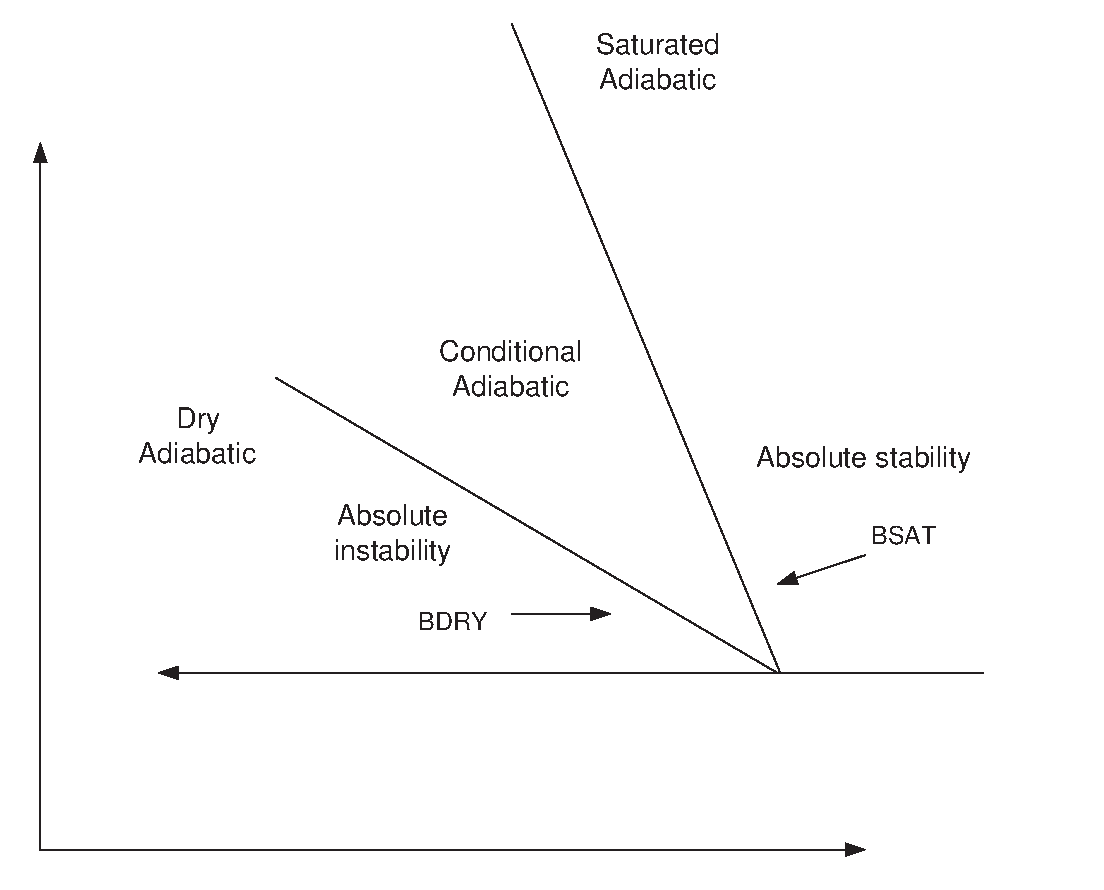
\includegraphics[width=11cm]{vertstab.eps}
    \caption{Stability conditions for the vertical stability of saturated and unsaturated air.} %this is how it shows up in the List of Figures
    \label{f:verticalstab}
    \end{figure}
.\\    
And finally I end this example file with a table which will be centered in the middle of the following page
\begin{table}[hp]
\centering
\renewcommand{\arraystretch}{1.5}
\begin{tabular}{|ll|}
\hline
\multicolumn{2}{|c|}{\bf\sffamily {\it Data} files listed in a table }\\
\hline\hline
\multicolumn{2}{|l|}{\bf\sffamily First part} \\
Fabracadabra.m	& - Saturation computation\\
Fobracadabra.m	& - Pressure computation\\
Fibricadibri.m	& - Permeability computation\\
&\\
\multicolumn{2}{|l|}{\bf\sffamily Structural rock model} \\
struct.m	& - Rock structural data using symmetric boundary condition \\
bstruct.m	& - Rock structural data using anti-symmetric boundary condition \\
\hline
\end{tabular}
\caption{Good-looking program data deck files.} %this is how it shows up in the List of Tables
\label{tbl:tbl}
\end{table}





%
% Bibliography
    \bibliographystyle{apalike}
    \printbib{MyBib} % in MyBib.bib you add all your reference information, following the correct format.
    % The *.bin file needs to be compiled using the Bib-compile option of your LaTeX text editor. Sometimes, the bib file needs to be built several times, as well as the main file, before all references occur correctly in your PDF.


%============================= Back matter =========================================
\appendix

    \chapter{The back of the thesis}

    \section{An appendix section}

    \subsection{An appendix subsection with C++ Lisitng}

    \lstset{language=C++}
    \lstinputlisting{test.c}

    \subsection{A \matlab $ $ Listing}

    \lstset{language=matlab}
    \lstinputlisting{test.m}

    \chapter{Yet another appendix}

    \section{Another test section}

    Ok, all is well.

% Index
    \printindex
    \cleardoublepage

\end{document}

